\section{[Complete] Packet-based Serial Communication}
In this project, I tried to communicate with the VEX Cortex via a Raspberry Pi by sending it packets of data via their UART serial ports \cite{UARTBasic}; This is an inspiration from EvolvedAwesome's VEXSerial \cite{VEXSerial} -- a basic, pretty messy library for this exact purpose. I took it one step further and made my own library for serial communication, so that it'd work with a webserver as well.

\begin{figure}[h]
    \centering
    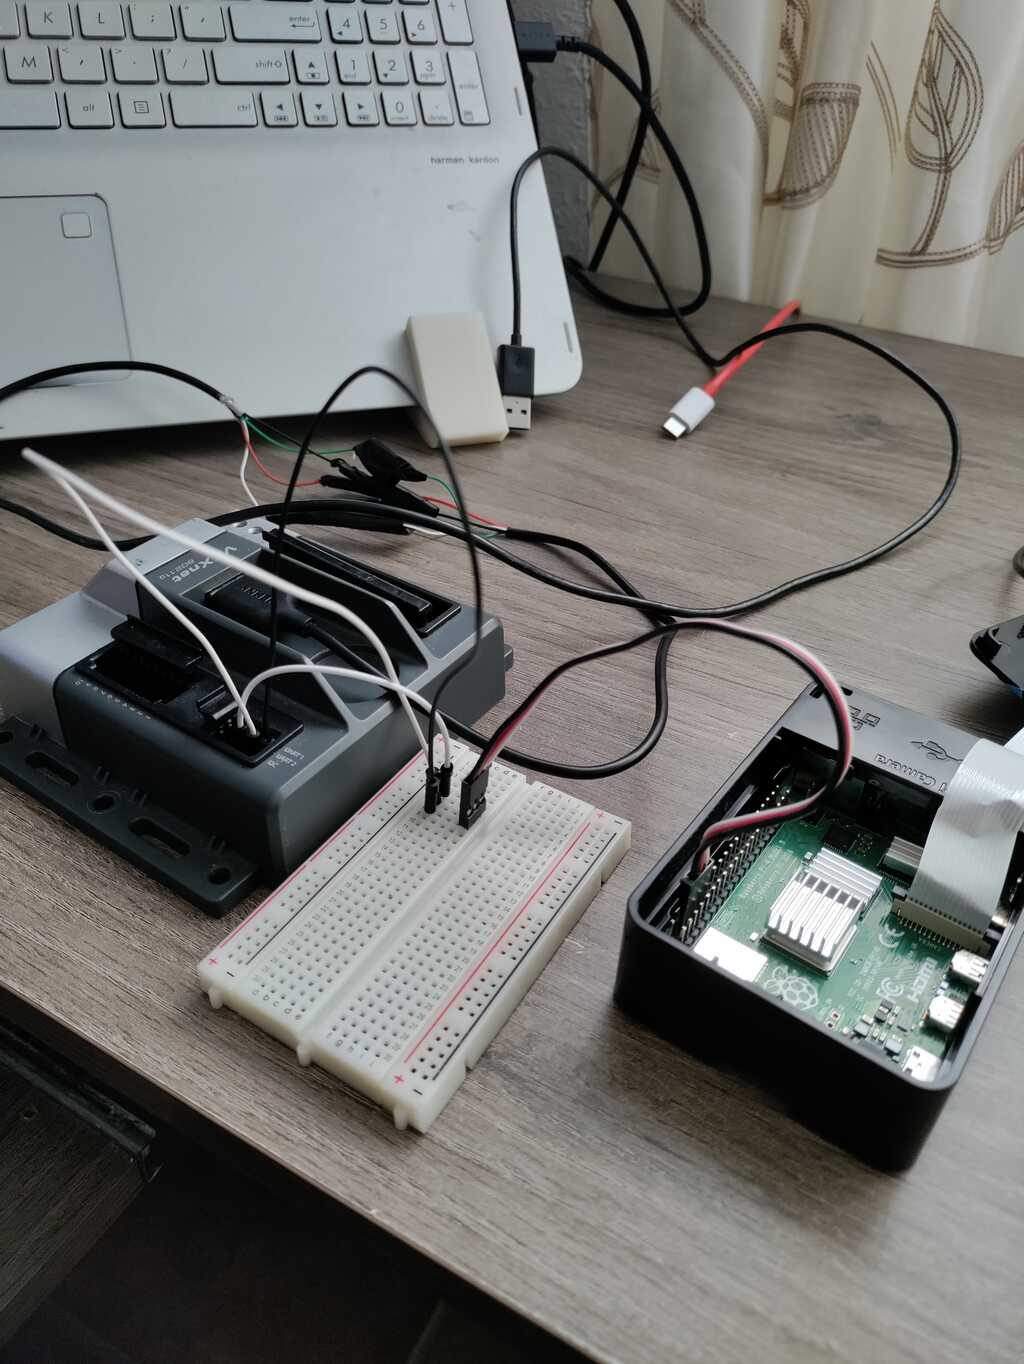
\includegraphics[width=\textwidth,height=6cm,keepaspectratio=true]{SerialSetup}
    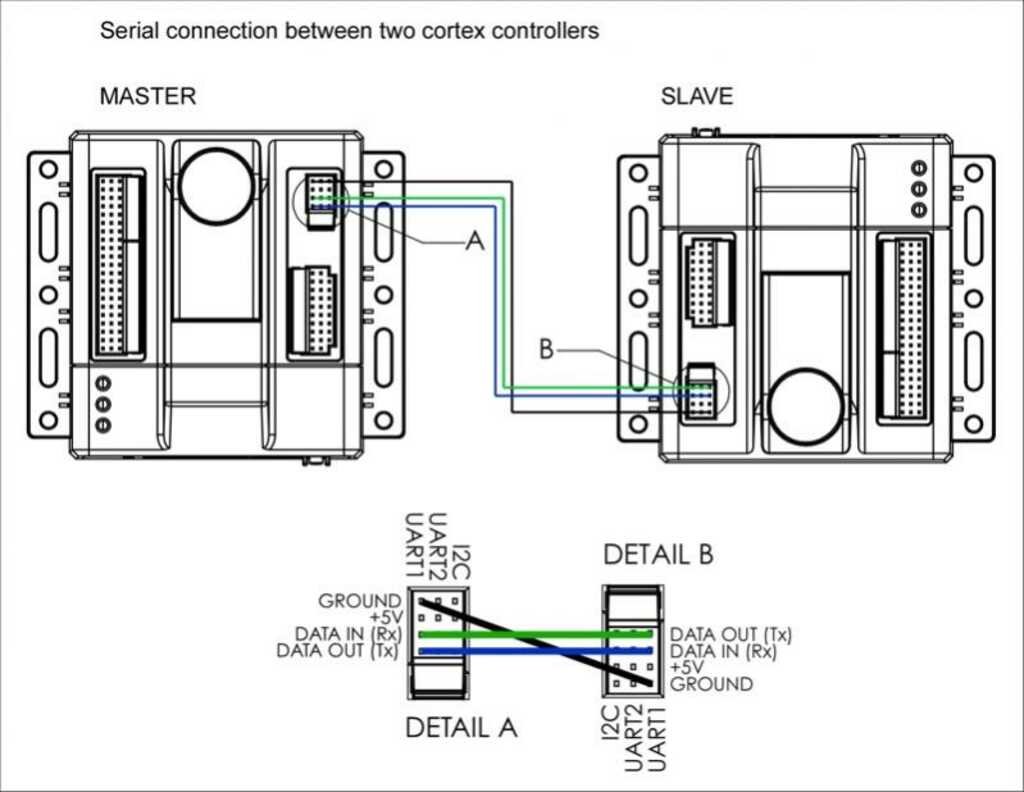
\includegraphics[width=\textwidth,height=6cm,keepaspectratio=true]{CortexWiring}
    \caption{
        (Left) The Raspberry Pi being electronically connected to the VEX Cortex via jumper wires and a breadboard. (Right) Diagram showing the UART ports of the Cortex. \cite{CortexWiringCite}
    }
\end{figure}

For our purposes, the idea was to have a python program on a Raspberry Pi send serial data to the cortex based on controller input over a HTTP server. This way, the robot can be completely controlled by the Raspberry Pi over any remote computer, no VEXnet controller needed. If one were to also use the Raspberry Pi as a camera, you have yourself an RC car with a cheap wireless FPV system.

\begin{figure}[h]
    \centering

    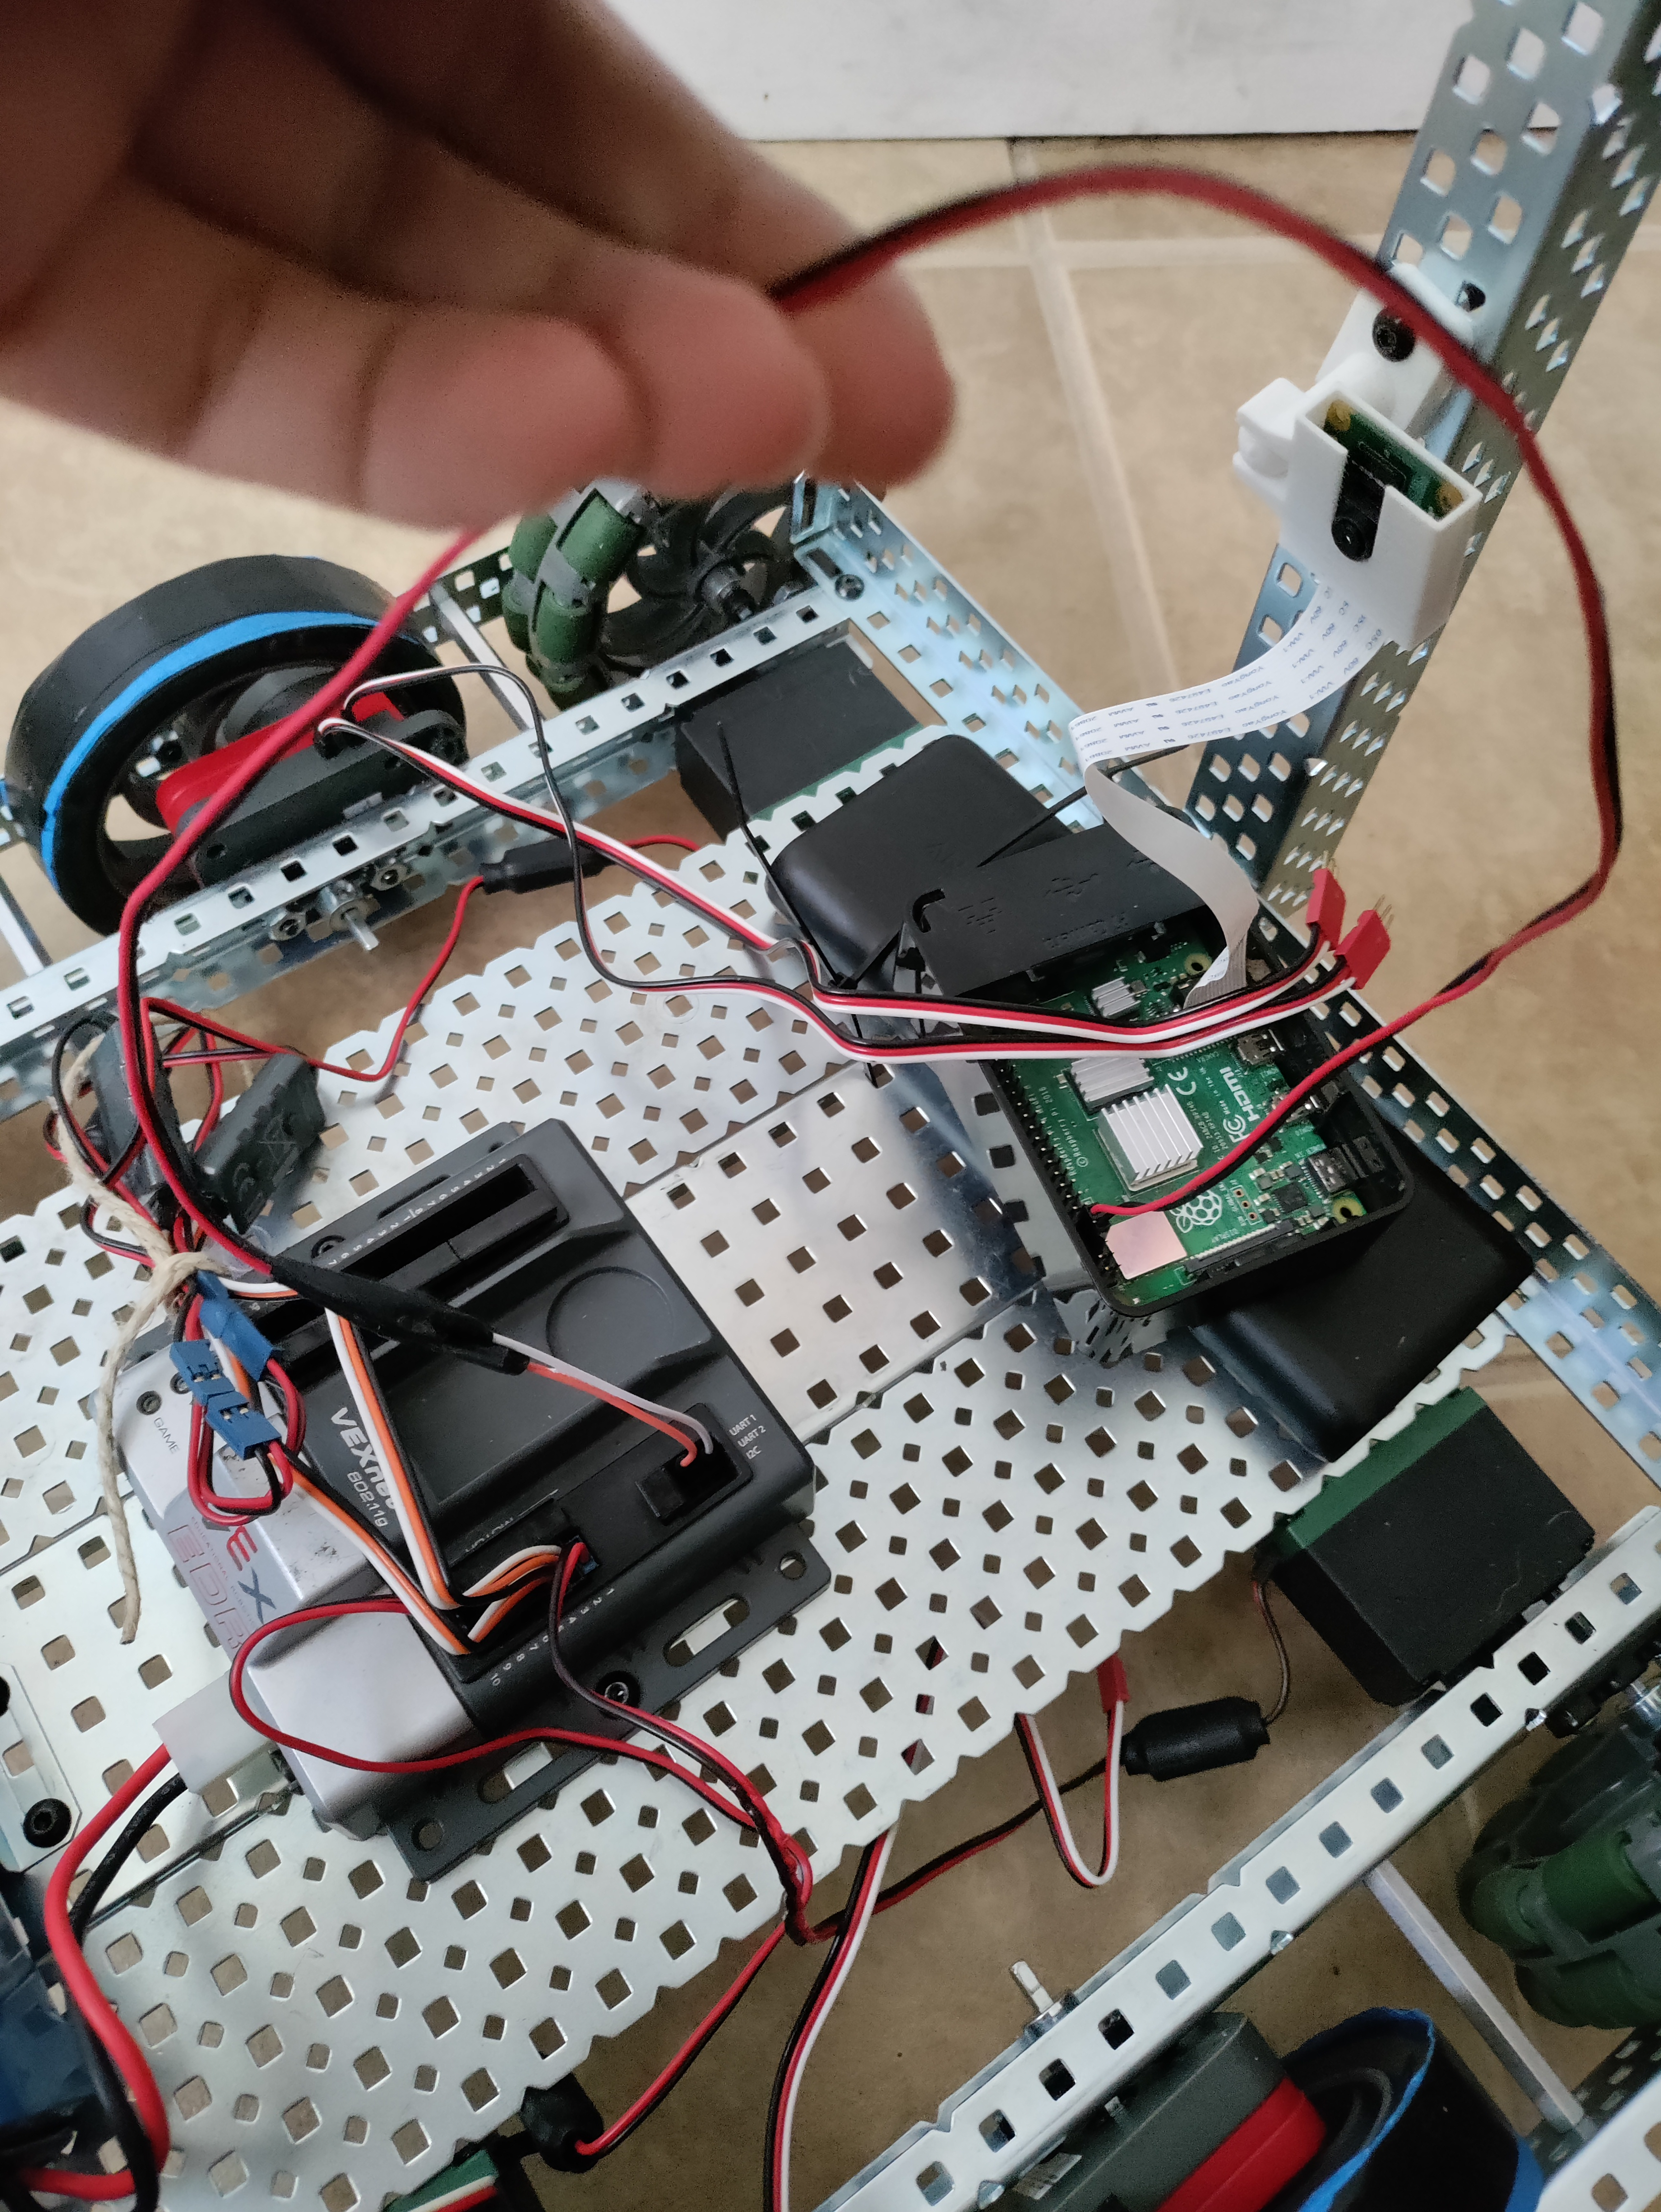
\includegraphics[width=\textwidth,height=6cm,keepaspectratio=true]{SerialMounted}
    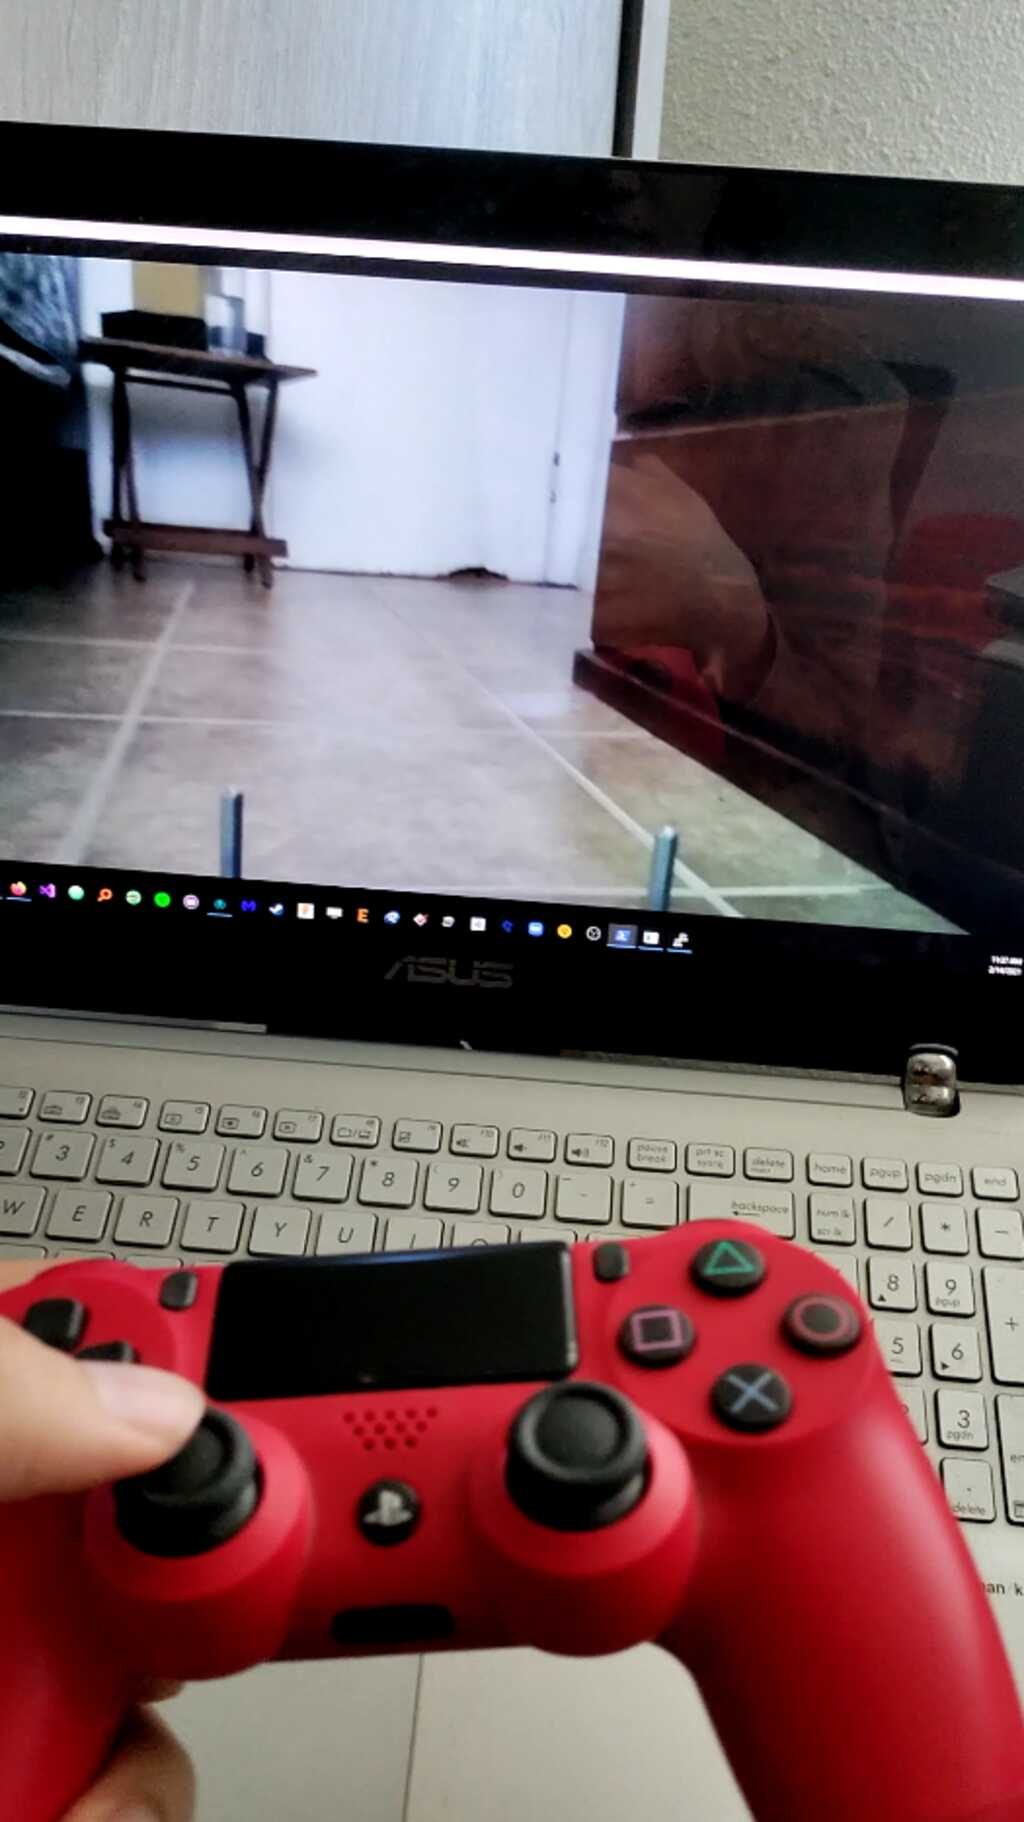
\includegraphics[width=\textwidth,height=6cm,keepaspectratio=true]{RemoteController}
    \caption {
        (Left) The setup mounted on the robot in combination to a camera; The electronic link between the Raspberry Pi and Cortex was made using a homemade female to male connector, making the use of a breadboard unnecessary. (Right) A photo of the robot being controlled by a PS4 controller in addition to real-time video feed.
    }
\end{figure}

So I did just that. I looked up the wire configuration of both the Raspberry Pi and Cortex, linked them together electronically, and made code to test if serial code can be sent in the first place. After that, I implemented a packet-backed system in RobotC that allowed me to completely mimic all inputs made on a regular VEX controller using just 4 bytes, or 32 bits. I then tried it out on a mobile hotspot for maximum bandwidth and signal strength, and the result is perfect.

This system allowed me to reach 2-3x farther distances compared to a VEXnet controller due to a packet switcher now amplifying the strength of the signal. The code is also set up in a way where, in case of any disconnect, the Raspberry Pi will seamlessly connect back to the transmitter; Just like any regular controller. If we ever want to control the robot wirelessly over colossal distances, we can also buy a dedicated router, connect it to a computer via ethernet, and simply move the router near wherever the robot will usually be and have the ethernet cable bring signal to our computer.
